\documentclass[11pt, preprint]{aastex}
%%%%%%begin preamble
\usepackage[hmargin=1in, vmargin=1in]{geometry} % Margins
\usepackage{hyperref}
\usepackage{url}
\usepackage{natbib}
\setlength{\bibsep}{0pt plus 0.3ex}
\usepackage{graphicx}
\usepackage{amsmath}
\usepackage{amsfonts}
\usepackage{amssymb}
\usepackage{pdfpages} % breaks with aastex6
\usepackage{import}
\usepackage{wrapfig}

\usepackage{color}
\hypersetup{
  colorlinks   = true,
  %citecolor    = blue
  citecolor    = gray
  % gray is not being found!?!
  % gray is found if pdfpages is used... crap.
  %citecolor    = grey
  %citecolor    = Gray
}

\setcounter{tocdepth}{2}
%% headers
\usepackage{fancyhdr}
\pagestyle{fancy}
\fancyhf{} % sets both header and footer to nothing
\lhead{Evan Anders -- Research Proposal}
\rhead{Princeton Center for Theoretical Science}
\cfoot{\footnotesize{\thepage}}
%\pagestyle{empty}
%\pagenumbering{gobble}
%\renewcommand*{\thefootnote}{\fnsymbol{footnote}}

\renewcommand{\vec}{\ensuremath{\boldsymbol}}
\newcommand{\dedalus}{\href{http://dedalus-project.org}{Dedalus}}
\newcommand{\del}{\ensuremath{\vec{\nabla}}}
\newcommand{\scrS}{\ensuremath{\mathcal{S}}}

\newcommand{\nosection}[1]{%
  \refstepcounter{section}%
  \addcontentsline{toc}{section}{\protect\numberline{\thesection}#1}%
  \markright{#1}}
\newcommand{\nosubsection}[1]{%
  \refstepcounter{subsection}%
  \addcontentsline{toc}{subsection}{\protect\numberline{\thesubsection}#1}%
  \markright{#1}}

%\usepackage{atbegshi}
%%%%%%end preamble


\begin{document}
Stars like the Sun rely on vigorous near-surface convective regions to transport out the heat generated in their cores.
This convection generates sound waves which deflect due to density stratification as they propagate into the stellar interior.
The relatively new fields of helio- and asteroseismology measure those sound waves to look into the interior of the Sun and other stars.
These measurements enable the precise determination of age, mass, and radius of other stars, and have revealed the interior structure and mean flows of the solar interior.
These helioseismic observations, as well as direct measurements of the Sun's surface, have been unable to detect theorized large-scale convective flows called ``giant cells'' within the Sun.
The absence of these flows have called into question our most fundamental understanding of the nature of convection in stars, a problem widely referred to as the ``Solar Convective Conundrum.''

State-of-the-art simulations used to generate the internal structure of stars often rely on simple parameterizations of convection.
These stellar structure models are used widely across many subfields of astrophysics, including the aformentioned asteroseismology.
However, the convective parameterizations that inform these codes predict the presence of giant cells in the Sun, which we do not see in numerous observations.
My research focuses on using novel theoretical and computational tools to better understand the nature of convection in the highly stratified, magnetized, rotational context of stellar convection in order to help solve this Convective Conundrum.
While my motivations are focused on the Sun and stars, similar processes are important in the atmospheres and cores of planets, including the Earth. 

\section{Entropy Rain: Downflows in stellar convection}
\vspace{-6pt}

In the presence of an atmospheric density stratification, convective flows experience a breaking of symmetry.
That is, upflows become slow and broad while downflows become intense, fast, and narrow.
It has been suggested that in the context of solar-like convection, these intense downflows are so powerful that they do not require their upflow counterpart to carry out the Sun's luminosity.
This ``entropy rain'' hypothesis, first suggested by \citet{spruit1997}, is gaining traction, and could explain the lack of large-scale upflows in observations \citep{hanasoge&all2015}.
\begin{wrapfigure}{r}{0.4\textwidth}
	\begin{center}
	\vspace{-10pt}
    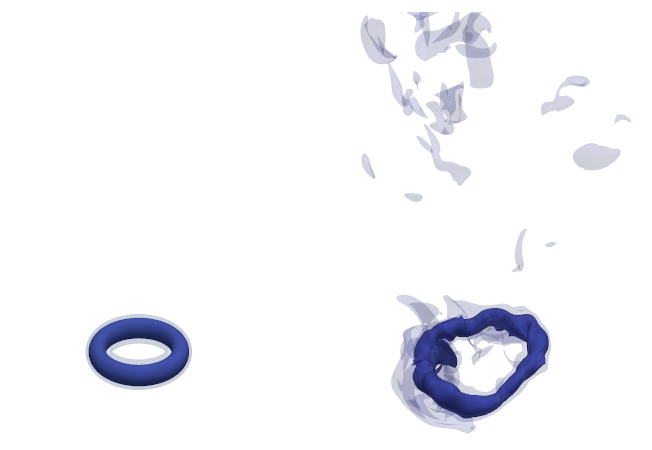
\includegraphics[width=0.38\textwidth]{./figs/thermals_comparison.png}
	\vspace{-16pt}
	\end{center}
    \caption{
	3D visualizations of the entropy perturbation of evolved thermals in the laminar (left) and turbulent (right) regimes.
	\label{fig:thermals_comparison} }
	\vspace{-11pt}
\end{wrapfigure}
Recent simulations of solar-like convection have hinted that downflows may be the primary driver of this stratified convection \citep{kapyla&all2017}, and recent theoretical work showed that such a concept could be included into our simple parameterizations \citep{brandenburg2016}.
As a result, the nature of downflows in stellar convection deserves a more careful study; these downflows may turbulently break up into distinct pieces as they fall and these pieces can be modeled as ``thermals.''
Thermals are regions of cold fluid which accelerate due to buoyancy forces and shape themselves into vortex rings; evolved thermals are visualized in Fig. \ref{fig:thermals_comparison}.
Thermals are also observed and studied in the Earth's atmosphere \citep{lecoanet&jeevanjee2019}.

Over the course of my graduate studies, I have become proficient at using the open-source Dedalus \citep{burns&all2019} code to answer questions about stellar convection at various scales.
During my PhD, I used Dedalus to study thermals-as-downflows by coming to understand how atmospheric stratification affects these downflows as they fall \citep{andersLB2019}.
In the absence of stratification, thermals expand and stall as they propagate \citep{lecoanet&jeevanjee2019}; the inclusion of stratification allows thermals to compress and accelerate as they fall, but they do not compress as intensely as simple arguments would expect \citep{brandenburg2016}.
We found, to our surprise, that solar downflows could easily carry the solar luminosity through these cold, raindrop-like downflows without any help from warm upflows, giving credence to the entropy rain hypothesis.
However, these studies neglected three key ingredients in stellar convection which should be explored: turbulence, magnetism, and rotation.

As a PCTS fellow, I will build upon this study from my thesis work to understand if entropy rain is feasible by including solar-like complications.
At certain latitudes, rotationally-induced Coriolis forces could likely deflect these raindrops before they transit the solar convection zone.
Magnetic interactions could have similar filtering affects, keeping a large fraction of these rain droplets from reaching the base of the convection zone.
While \citet{lecoanet&jeevanjee2019} found that turbulence had little effect on thermals in unstratified atmospheres, the compressional effects of atmospheric stratification could change this outcome.
If the inclusion of these complications prevent downflows from crossing the solar convection zone, then it is clear that such a mechanism cannot be responsible for carrying out the Sun's energy.
These careful studies will determine which regimes, and for which stars, Entropy Rain could be an important mechanism.
As in \citet{andersLB2019}, these studies will include both analytical and numerical analysis.
I look forward to collaborating with experts in theoretical fluid dynamics like Prof.~Jeremy Goodman.
I further look forward to collaborations with the experts in Princeton's Geophysical Fluid Dynamics laboratory, who study convection in the context of Earth's atmosphere where thermals are observed.



\vspace{-0.8cm}
\section{Downflow interactions at the radiative-convective boundary}
\vspace{-0.3cm}
\label{sct:taskB}
\begin{figure*}[t!]
    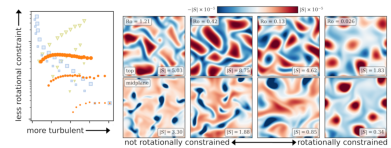
\includegraphics[width=\textwidth]{./figs/rossby_plot.png}
    \caption{(left, Fig 1b of \citet{anders&all2019}) The degree of rotational constraint is difficult to predict as a function of turbulence in convective simulations.
	Along traditional paths through parameter space (green triangles and blue squares), rotational constraint varies strongly as a function of turbulence.
	However, when our newly discovered ``predictive Rossby number'' is held constant (orange circles), the degree of rotational constraint can be held constant while turbulence is increased.
	(right eight panels, Fig. 2 of \citet{anders&all2019}) As rotational constraint increases (from left to right), traditional granular convective patterns give way to quasi-two-dimensional vortical columns of convection with very little difference between the top of the atmosphere and the atmospheric midplane (top row vs. bottom row).
	Rotational constraint modifies convective dynamics, so simulating in the proper rotational regime that reflects the Sun or another star being studied is crucial.
	\label{fig:rossby_plot} }
\end{figure*}

In Sun-like stars, beneath the turbulent surface convection zone lies a stably stratified ``radiative zone'' where radiation effectively carries out the Sun's heat.
In the Sun, the radiative-convective boundary (RCB) is characterized by a transition from moderate instability to strong stability.
The solar RCB furthermore coincides with a region of intense shear in the Sun's radial velocity profile called the tachocline, and it is thought that these shear interactions are a crucial driver of the Sun's magnetic dynamo.
Understanding how downflows pump angular momentum and magnetism into the RCB is crucial for understanding both the solar dynamo and the latitudinal differential rotation profile of the Sun.
Measurements suggest that the RCB is thin \citep{basu1997}, but many modern simulations produce RCBs which are up to an order of magnitude thicker than the solar one.
This suggests that many simulations are studying angular momentum and magnetic field pumping mechanisms in the wrong regime of ``stiffness'' of the RCB \citep{couston&all2017}.

While studying convection in the Sun, it is important to study flows who feel the same influence of rotation and magnetism as they do in the Sun.
In a convective simulation which includes an effect like global rotation, simulations can be run in a regime where flows are heavily affected by Coriolis forces or a regime where this effect is weak.
A ``critical'' rotational frequency separates these two regimes, but determining this critical frequency is often not straightforward.
During my graduate career, I found a method for determining this frequency so that the importance of rotation on the evolved nonlinear state could be specified in simulation initial conditions \citep[see Fig. \ref{fig:rossby_plot} and][]{anders&all2019}.
In magnetized systems, there is an analagous critical magnetic field, but to date no study has determined how to determine this field before simulation startup.

During my time at PCTS, I will study the interactions of downflows in the appropriate rotational and magnetic regime as those in the Sun.
In order to achieve this, I will first determine the critical magnetic field using similar techniques to those that I used during my graduate career while finding the critical rotational frequency.
After determining this, I will study rotating magnetoconvection in the same flow regime as solar convection, and come to understand how effectively downflows pump magnetic fields and angular velocity into a solar-like RCB.
These studies wll greatly benefit from partnerships with experts in astrophysical fluid dynamics at Princeton and the IAS like Profs.~Jim Stone and Matthew Kunz.

\section{Global studies in relaxed atmospheres}
Modern stellar models often employ the decades-old convective parameterization of mixing length theory \citep{bohm-vitense1958}, which has many deficiencies.
These deficiencies have led some researchers to seek out ways to couple one-dimensional (1D) models with fully convective, three-dimensional (3D) global simulations.
Such a coupling has recently been performed with some success \citep{jorgensen&weiss2019}.
These studies have thusfar only been able to couple previously computed 3D sims with 1D models, rather than coupling the two at runtime.
This is largely because 3D simulations are costly.
Some of these costs are unavoidable: highly resolved, turbulent simulations necessarily take small timesteps, and therefore simulation times are very long.
However, some of the expense of these simulations is often time wasted waiting for the atmospheric structure and mean flows to converge to an equilibrium state, and this expense can be minimized.

\begin{wrapfigure}{r}{0.3\textwidth}
	\begin{center}
	\vspace{-10pt}
    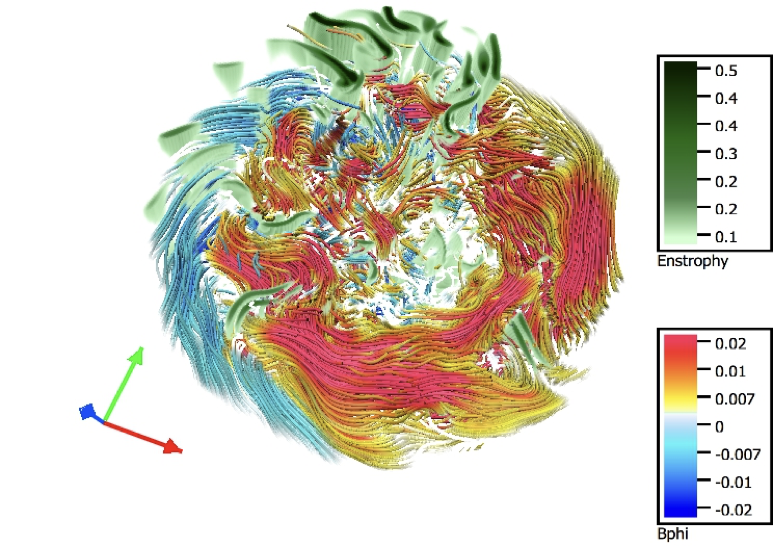
\includegraphics[width=0.28\textwidth]{./figs/mdwarf.png}
	\vspace{-16pt}
	\end{center}
    \caption{A volume rendering of a global dynamo simulation in Dedalus.
	Enstrophy, or the magnitude of vorticity, is shown in green.
	Red and blue lines denote the magnitude and direction of azimuthal magnetic field.
	\label{fig:mdwarf} }
\end{wrapfigure}
During my graduate career, I created and verified a tool for accelerating the long thermal relaxation timescale in convective systems \citep{anders&all2018}.
This tool reached a relaxed state using an order of magnitude fewer computational resources than when waiting for a standard thermal relaxation timescale.
During my time at PCTS, I will extend my accelerated evolution method to the evolution of thermodynamic and angular momentum profiles in global simulations.
The tools to perform global simulations in Dedalus already exist \citep{lecoanet&all2018} and have been tested; a visualization of basic outputs from these simulations is shown in Fig. \ref{fig:mdwarf}.
Once this global simulation accelerated evolution module is created, it will be made public, and will be designed so as to flexibly interact with arbitrary simulation data so that users of codes beyond Dedalus can benefit from the computational speed-ups of this tool.
I will also use this tool to accelerate the evolution of solar-like simulations to understand the nature of global flows and dynamos in relaxed simulations.

\vspace{-0.8cm}
\section{Summary}
\vspace{-0.3cm}
The Princeton Center for Theoretical Science postdoctoral fellowship would give me the freedom to study these ambitious problems in astrophysical fluid dynamics.
During my fellowship, I would study the interactions of convection, magnetism, and rotation in the context of the Sun, including the nature of the smallest flows and their interactions at the largest, global scales.
The results of these studies will inform stellar models  at a time when improving their results will be impactful for a variety of astrophysical disciplines.
Princeton is the perfect location for carrying out this work due to the opportunities available for interdisciplinary collaboration between astrophysicists, geophysical fluid dynamicists, and applied mathematicians.
I look forward to the opportunity to join the center and learn about the diverse work of the other fellows in theoretical sciences.

\newpage
\bibliographystyle{apj_title}
\bibliography{biblio}
\end{document}
